\section{RoPE}

\begin{frame}{Transformer}
    \begin{itemize}
        \item 记 $S_N = \left\{ w_i \right\}_{i=1}^{N} $ 是$N$个输入词汇序列
        \item $E_N=\left\{ x_i \right\}_{i=1}^{N}$ 是对应的 word embedding, $x_i$中没有位置信息
        \item 融入位置信息:
        \[
            \begin{cases} q_m &= f_q(x_m, m) \\ k_n &= f_k(x_n, n) \\ q_n &= f_v(x_n, n) \end{cases}
        \]
        \item attention weight: $a_{mn} = \frac{\exp(q_m^{T}k_n) / \sqrt d}{ \sum_{j=1}^{N}\exp(q_m^{T}k_j) / \sqrt d}$
        \item output embedding: $o_m = \sum_{n=1}^{N} a_{mn} v_n$
    \end{itemize}
\end{frame}

\begin{frame}{Rotary Position Embedding (a.k.a. RoPE)}
    \begin{itemize}
        \item 在 Transformer 模型中,RoPE 是一种将token位置融入 attention 模块的方法。
        \item 核心思想:希望计算 attention weight 的时候 $q_m^{T} k_n$ 点积结果只与 $x_m, x_n$ 和 $m-n$ 相关。
        \item 2D 情况下,一个解为复数解,可以等价地写成矩阵形式方便计算。
        \begin{center}
            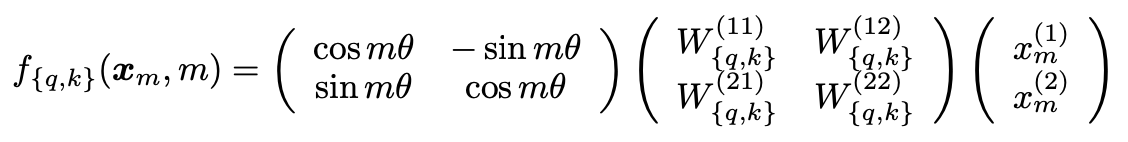
\includegraphics[width=0.6\textwidth]{assets/rope2.png}
        \end{center}
        \item 更高维情况下可以写成
        \begin{center}
            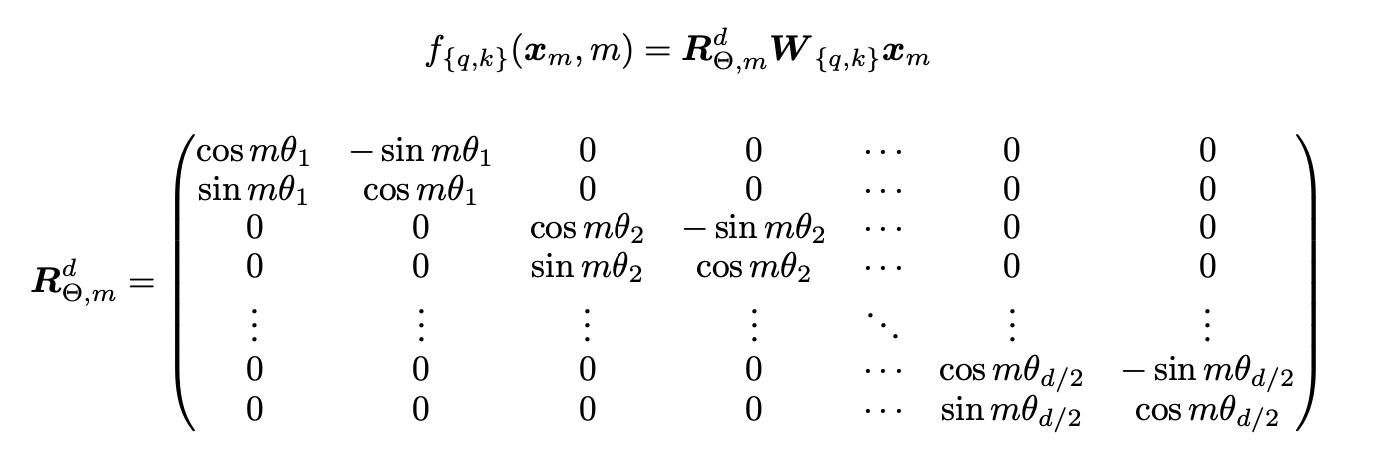
\includegraphics[width=0.5\textwidth]{assets/roped.png}
        \end{center}
        其中 $\Theta = \left\{ \theta_i = 10000^{-2(i-1)/d}, i \in [1, 2, \cdots, d / 2] \right\} $
    \end{itemize}
\end{frame}
